%===================================== CHAP 6 =================================

\chapter{Phase 2:  Application implementation}
\label{chap:phase2}

After the exploratory phase 1, phase 2 is more concerned with gathering concrete data. Functional requirements have been revised as a result of data gathered in phase 1, and more focus will be placed on creating a solid foundation as one of the major artefacts of the project. As the data in phase 1 indicated strongly toward a preference for multi-user experiences for workplace training, phase 2 can proceed mostly as planned.

By spending a lot of time with the tools selected for the project in the first phase, it has become apparent as to why a general solution is needed. While some custom logic will always be needed, the overarching plan for the NAV project is to create a \textit{workplace experience catalogue} that will allow users to browse workplaces as needed. It is therefore paramount that the experience is the same to satisfy user expectations. A general solution will also produce clearer results that are not muddied by having different parts of the application respond, operate or appear differently. Less time can be spent creating fundamental logic, and more time spent on making sure that the custom logic parts work well.

With this mind, the development work can be said to be split into two parts. One part will concern itself will implementing and creating a fully functional multi-user workplace experience as one of the two primary artefacts of the project. The other artefact and effort will be devoted to creating the general framework and mapping the process needed to convert a workplace experience to multi-user environment. As the artefacts created here will serve as a foundation for further development and research, a significant portion of time has been spent making sure that the artefacts created are up to the IMTEL lab standards, as well as following software architecture principles. In section \ref{section:Phase2Implentation} the details of this process will be explained. The following sections will detail the specific changes made to the artefact concerning the fully implemented workplace and an evaluation the artefact created.


\section{Planning and Changes}


\subsection{Changes}
The changes to the application is based mostly on the analysis done in the previous phase. From table \ref{table:themesInterview1} we presented sub-themes which after some internal discussion resulted in an agreement (which we felt covered the most important aspects) that we should add the following changes to this phase's development and implementation process. 

\begin{description}
    \item [Change 1]\hfill \\
    A fully functional virtual workplace environment which support multi-user functionality. Meaning objects, avatars, movement etc. should be networked and other data should be serialised in data streams to and from servers. 
    \item [Change 2]\hfill \\
    Direct communication so that users has the possibility to talk to each other. With voice chat users should only hear others talk, not themselves, avoiding echo and misinterpretations.  
    \item [Change 3]\hfill \\
    Collaborative features should be available for VR users, such as hand gesticulation and a laser pointer to pinpoint or mark objects.
    \item [Change 4]\hfill \\
    More realistic avatars with some aspect of personalisation. 
\end{description}





\subsection{Updated Requirements}
As mentioned above this phase adds several changes to the artefact. The requirements outlined in bold are additions for this phase.

\begin{enumerate}
  \setlength\itemsep{0em}
  \item [\textbf{F1}] The applications must allow multiple players to join the same scene.
  \item [\textbf{F2}] Interactable objects must be serialised and and synchronised over the network.
  \item [\textbf{F3}] A player shall be represented as an avatar with corresponding movement from the real world to the VR world.
  \item [\textbf{F4}] The application must offer the option of using VR equipment or desktop mode (mouse and keyboard) for interaction.
  \item [\textbf{F5}] The application must contain a scene with tasks enabling collaborative learning.
  \item [\textbf{F6}] The multiplayer component must be generalisable and scalable to work with other NAV applications.
  \item [\textbf{F7}] \textbf{The application must be a virtual workplace with multi user functionality}.
  \item [\textbf{F8}] \textbf{Users should be able to communicate through integrated voice chat functionality}.
   \item [\textbf{F9}] \textbf{VR users should be able use tool(s) to mark or pinpoint objects or locations}.
\end{enumerate}

\subsection{Development Decisions}
The largest difference between phase one and phase two is the environment and the tasks available to the users. While phase one focused on a functional multi-user implementation to showcase possibilities and to see that users could navigate and understand a collaborative VR environment, phase two is about creating a functional collaborative workplace. With this, the goal is to create an artefact that is as close as possible to what would be used in a normal use case, but with multi user functionality. 

For the virtual workplace to be used in this phase, a workplace developed at the IMTEL lab was chosen based on several criteria. Due to the time frame of the project, it was decided that a new workplace would not be created. Instead, the choice was made to use one already developed at the IMTEL lab, as that would allow us to ask questions to the developers regarding any issues that might occur. 

Secondly was the issue of scope and complexity. To properly test the possibilities of collaboration in VR, there needed to be a proper set of tasks that were neither to small nor too large. Too small, and the testers would finish it in no time, or the space might feel cramped. Too large, and there might be unforeseen issues implementing collaboration elements or for testers navigating the space together. Since the application would not be developed from the ground up, a larger and more complex application could also create issues when trying to serialise all the necessary information and states per task and player. Using more limited application would allow more time to work on individual serialisation to make sure that the application maintained consistency across the clients of all currently connected users. 

The recency of the workplace was also a concern. Due to the nature of the collaboration between the IMTEL lab and NAV, the developers of the older projects are not necessarily ready, or available at all, to help with issues, even if the application was made at the lab. As such, it would be helpful to use a fairly new workplace.

Considering these criteria, the newly developed car mechanic workplace was chosen. In this workplace, the users can attempt several different tasks in a garage, with the aim of introducing the user to some of the tasks a car mechanic might face in a normal workday \cite{IMTELinternships}.


\begin{figure}[H]
  \centering
    \captionsetup{width=1\linewidth}
    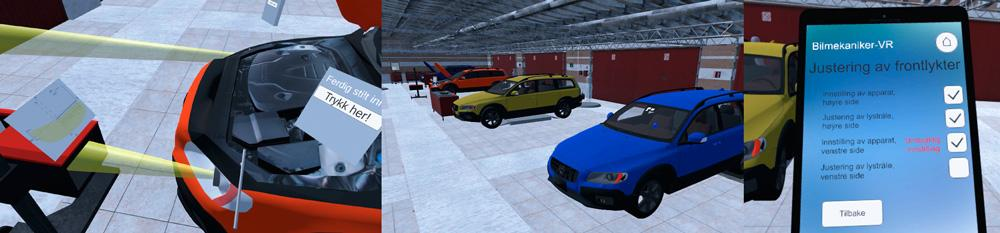
\includegraphics[width=1\textwidth]{fig/phase_2/Car-mechanic-app-screen.jpg}
    \caption{Screenshots of the car mechanic workplace application. \textit{Credit: IMTEL lab}}
\label{fig:Car-mechanic-app}
\end{figure}


\subsubsection{Virtual Reality}
In response to feedback, several decisions were made in this phase to enhance the experience of the individual users, and how they could interact in VR. This included altering the avatars to be less grey and dull, so that they would not blend into the environment as much. They were also given a hat so that their silhouette would be more distinct.  See figure \ref{fig:phase2Avatars}.
According  to  Wallach  et  al. it is possible that users of a VR application often focus on discordant elements in the VR environment rather than accurate element which might indicate that the feeling of presence is influenced by the existence of such discordant elements \cite{presenceInVirtualReality:}. A more realistic visual representation for a human as an avatar can therefore, as outlined in section \ref{section:socialPrecence}, contribute to an increased feeling of social presence. 

Finding a way to let players highlight either their own location or the location of a specific object was also taken into consideration. After some discussion, the decision was made to implement a form of laser pointer that can be activated for each player. The laser has significantly more accuracy than the standard hand, and can be used to pinpoint rather small objects. Example of use cases can be seen in figure \ref{fig:phase2Laser}.

Perhaps most important was the possibility of direct communication. To begin with, direct voice chat has been implemented in the application. An important consideration was the that audio quality had to be good with little to no background noise and echo as it can impact both the usability and the feeling of social presence (see section \ref{section:socialPrecence}) for the users. 
The effect on collaboration with voice chat would have to be investigated before adding more features to it, so certain Quality of Life features such as speech indicators or low fidelity animations to indicate speech could be implemented later based on time and further feedback. If users feel that it is hard to figure out who is talking, or where the other users are, the importance of these features can be adjusted to more accurately reflect their perceived value to the overall application.




\begin{figure}[]
  \centering
  \begin{subfigure}[b]{0.4\textwidth}
    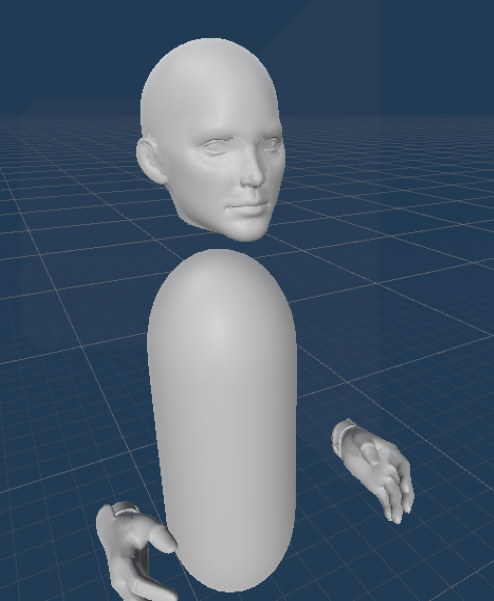
\includegraphics[width=1\textwidth]{fig/phase_2/implementation/oldAvatar1.png}
    \caption{The old avatar model from phase 1 with a grey colour schema.}
    \label{fig:oldAvatar}
  \end{subfigure}
    \hfill%
  \begin{subfigure}[b]{0.4\textwidth}
    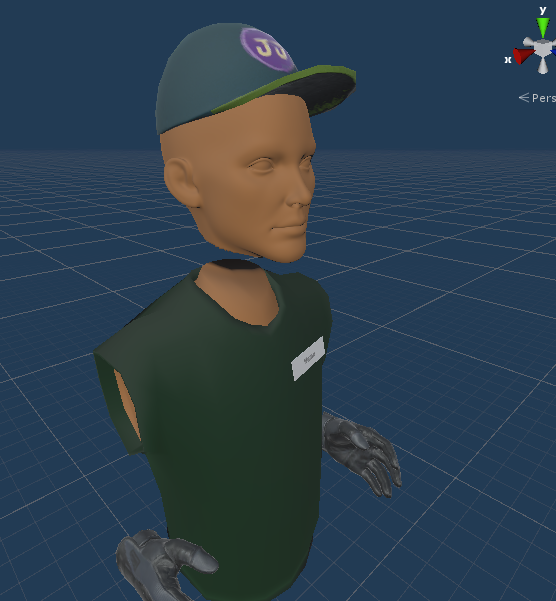
\includegraphics[width=1\textwidth]{fig/phase_2/implementation/avatarModel.PNG}
    \caption{The enhanced avatar model with more realistic colours, hat, gloves and name tag.}
    \label{fig:newAvatar}
  \end{subfigure}
  \hfill%
  \caption{Iterations of the avatar model.}
  \label{fig:phase2Avatars}
\end{figure}


\begin{figure}[]
  \centering
  \begin{subfigure}[b]{0.45\textwidth}
    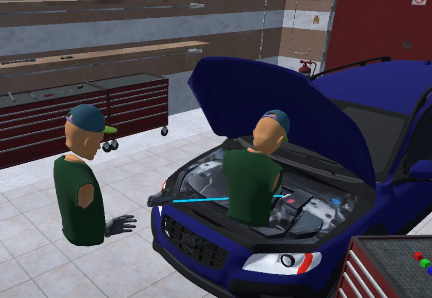
\includegraphics[width=1\textwidth]{fig/phase_2/implementation/laser1.png}
    \caption{A user pinpointing a loose hose in the engine compartment with the laser.}
    \label{fig:laser1}
  \end{subfigure}
    \hfill%
  \begin{subfigure}[b]{0.45\textwidth}
    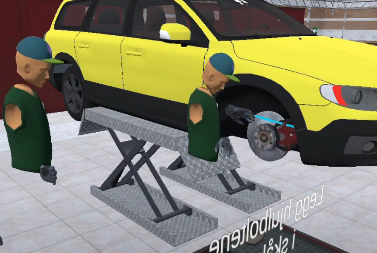
\includegraphics[width=1\textwidth]{fig/phase_2/implementation/laser2.PNG}
    \caption{A career counsellor highlighting a caliper bolt for the users who need help to complete the task.}
    \label{fig:laser2}
  \end{subfigure}
  \hfill%
  \caption{Laser pointer feature in action during testing.}
  \label{fig:phase2Laser}
\end{figure}


\section{Implementation}
\label{section:Phase2Implentation}
As the implementation got started, it was obvious that some sort of triage needed to be performed. The overall application was broken into its composite pieces, and to the highest degree possible, components were separated and isolated. Figure \ref{fig:highLevelArchitecture} illustrates the high level architecture of the application. In the case of the car mechanic application, it consisted of two main scenes, one small and one large. First was the wardrobe, where players had to equip the proper equipment before heading into the garage proper, see figure \ref{fig:wardrobeApp}.

\begin{figure}[H]
  \centering
    \captionsetup{width=1\linewidth}
    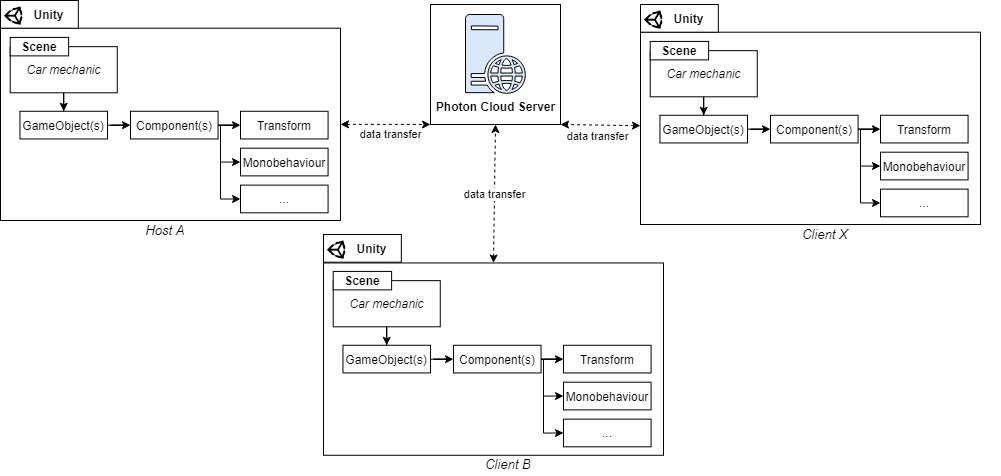
\includegraphics[width=1\textwidth]{fig/phase_2/implementation/highLevelArchitecture.jpg}
    \caption{High level diagram of the architecture.}
\label{fig:highLevelArchitecture}
\end{figure}


\begin{figure}[H]
  \centering
  \begin{subfigure}[b]{0.47\textwidth}
    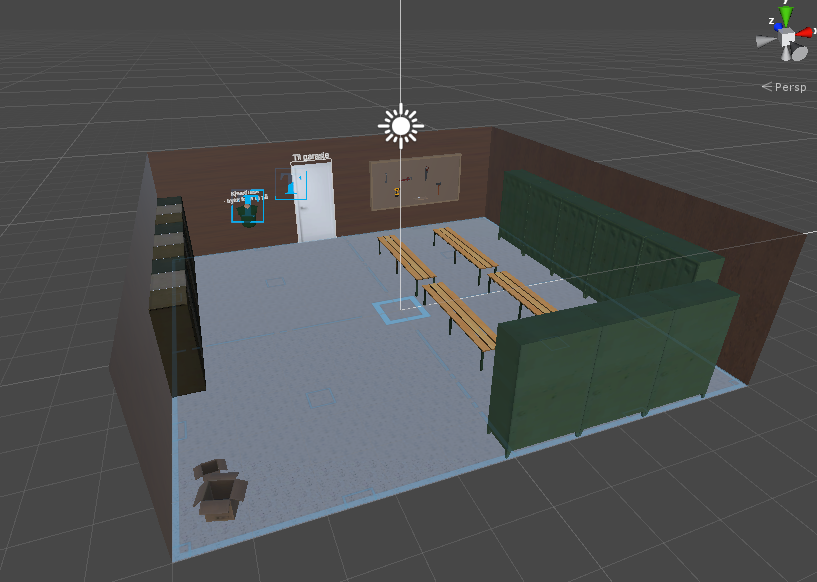
\includegraphics[width=1\textwidth]{fig/phase_2/implementation/wardrobe.PNG}
    \caption{Screenshot of the wardrobe model in Unity.}
    \label{fig:wardrobeApp}
  \end{subfigure}
  \hfill%
  \begin{subfigure}[b]{0.47\textwidth}
    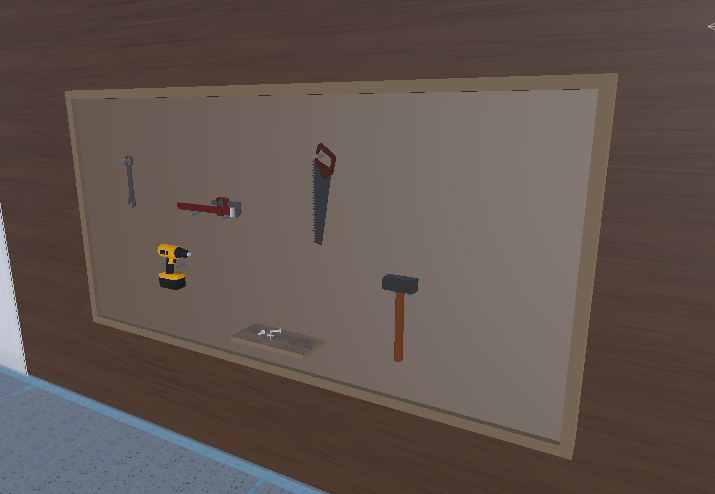
\includegraphics[width=1\textwidth]{fig/phase_2/implementation/toolsWall.PNG}
    \caption{Tool wall with different networked tools.}
    \label{fig:toolWall}
  \end{subfigure}
  \hfill%
  \caption{The wardrobe scene.}
  \label{fig:phase2Wardrobe}
\end{figure}


There was not too much happening here, so to begin with we made sure player instances and avatar representations were instantiated correctly in the room. We also added a simple wall with different tools that the awaiting users could interact with, adapting scripts for object networking and serialisation from phase 1, see figure \ref{fig:toolWall}. Other than that the last thing that was implemented was the ability for the multiple players to enter the garage through the door. Generally, in a online multiplayer game the master-client  handles scene changes, as was the case with standard PUN2 framework. We added logic in the network code so that whomever opens the door, even though it is not the master-client, and callback is sent to the the master-client telling a scene change needs to happened. It is an adaption of the software design pattern \textit{Observer Pattern}, where if one object is modified dependant objects gets notified.    



Once inside the garage, the meat of the matter becomes prevalent. The garage contains four separate cars that all have various tasks assigned to them, see figure \ref{fig:phase2Garage} for an overview. These were from the start designed separately, with no overlap, which made it easy to focus on one of them at a time. Making sure that each task worked over the network had varying degrees of complexity, largely dependant on the tasks' original complexity. For each of the task, understanding the code was essential. This led to some time being spent on each task simply breaking down the code and structure of each game object. Once thoroughly understood, the basic networking pieces could then be added, and the necessary components and scripts switched out for new, networked variants created in phase one (see chapter \ref{chap:phase1}). For those tasks that required further networking, or had some state that needed to be uniquely maintained, new scripts were created as required, while still aiming to maintain simplicity.  In so far as it was possible, adherence to certain principles was kept a high priority. 

In terms of software conventions we followed several design principles which included \textit{ modularisation}, \textit{high cohesion - low coupling} and \textit{ entity-component}. Unity already provides the entity-component patterns as default, where entities are instances of \textit{GameObjects} and they get their logic (interaction, movement etc.) by classes (scripts) extending the base class \textit{Component}. See figure \ref{fig:highLevelArchitecture}. These classes inherits some useful methods and operators. 
Modularisation refers to the principal of splitting and dividing the system into independent modules which gives the benefit of an easier system to understand and use, while allowing re-usage any number of times. Lastly, we tried to adhere to the high cohesion - low coupling principle which emphasis that classes should only do related things while being as independent of other classes as possible.    

As detailed in section \ref{section:pun2} we also used the \textit{client-server architecture} as our computing model. 

\begin{figure}[H]
  \centering
  \begin{subfigure}[b]{0.47\textwidth}
    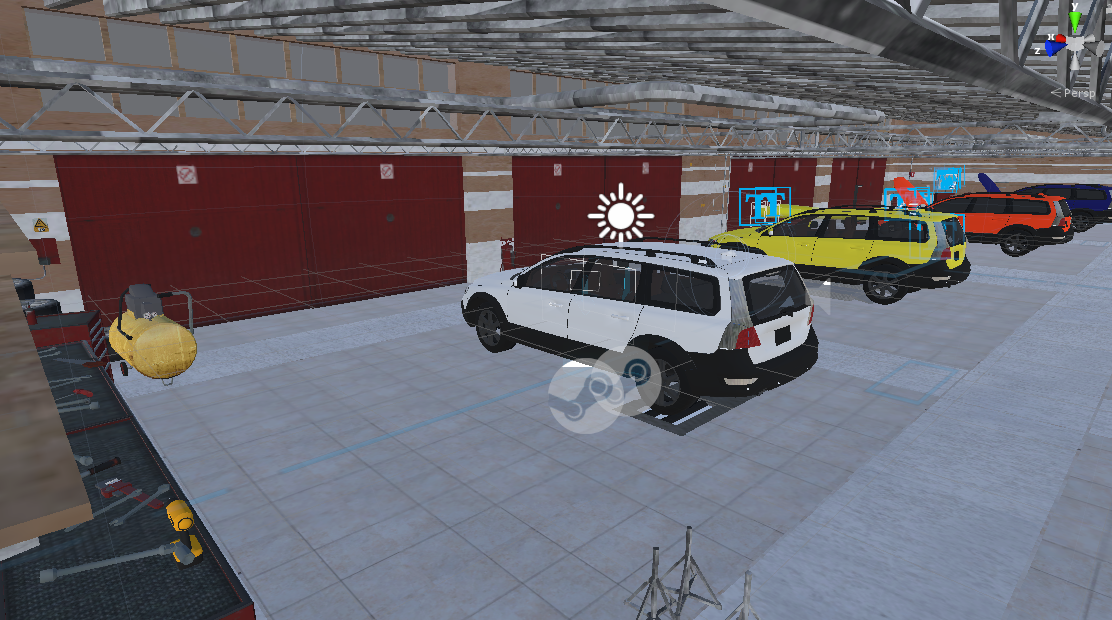
\includegraphics[width=1\textwidth]{fig/phase_2/implementation/workshop1.PNG}
    \caption{Screenshot from position of where the player objects are instantiated.}
    \label{fig:garage1}
  \end{subfigure}
  \hfill%
  \begin{subfigure}[b]{0.47\textwidth}
    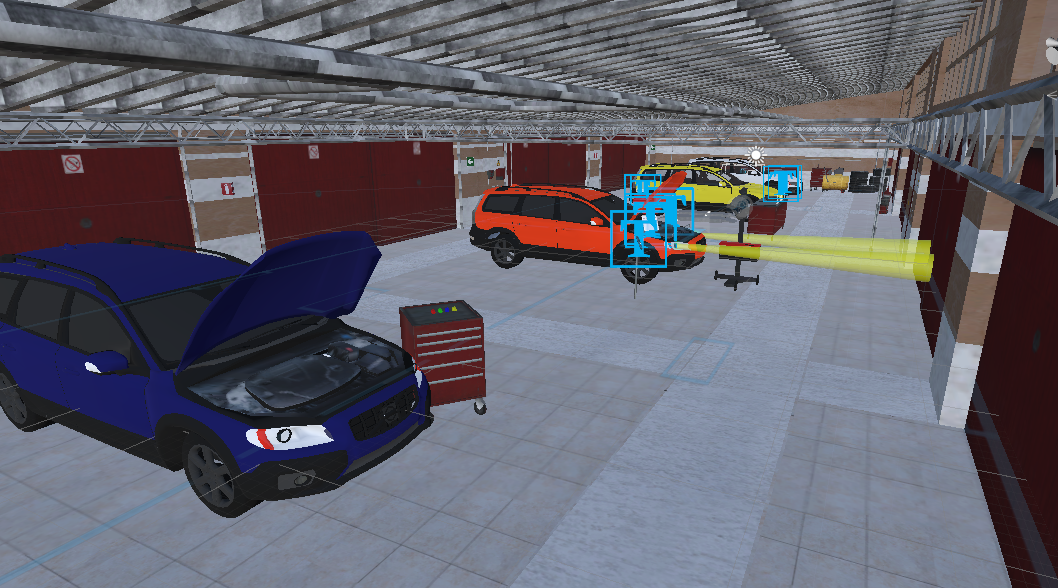
\includegraphics[width=1\textwidth]{fig/phase_2/implementation/workshop2.PNG}
    \caption{Screenshot from opposite side of the garage. Four cars with unique and realistic tasks.}
    \label{fig:garage2}
  \end{subfigure}
  \hfill%
  \caption{The garage scene.}
  \label{fig:phase2Garage}
\end{figure}


\subsection{Improving the serialisation of network objects}
For those objects that did not fit neatly into the basic entity types, it becomes necessary to create a \textit{PhotonView} script specific to that object that describes how the object is supposed to transfer its' data over the network to the other clients. When that is done, it is important to remember that since serialisation needs to be done manually, so does other things, like lag compensation. If the object also has triggers or other important changes that depend on user input, remote procedure calls from the Photon API can be very handy. It allows the player to request other clients to perform certain procedures remotely, hence the name. Using these RPCs, the state of the tasks can then be easily maintained across all clients, even with more complex state and triggers. A good example of the usefulness of an RPC method call is how it greatly simplified the serialisation of the complex car lift mechanism (see figure \ref{fig:carlift}). With this callback we could ignore the data serialisation for necessary states of the left and right piston, outer scissor and inner scissor mechanism, top plate and all other \textit{GameObjects} seen in figure \ref{fig:carliftTree}. Instead we call a method on remote players with one of three states: still (0), up (1) or down (-1). The local player then handles the rest with little alteration to original code.

\begin{figure}[H]
  \centering
  \begin{subfigure}[b]{0.61\textwidth}
    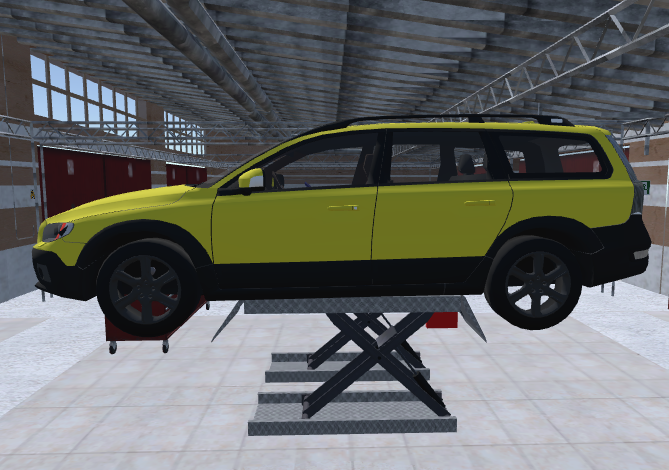
\includegraphics[width=1\textwidth]{fig/phase_2/implementation/carHoist.PNG}
 \caption{The car lift mechanism in the application.}
  \label{fig:carlift}
  \end{subfigure}
  \hfill%
  \begin{subfigure}[b]{0.28\textwidth}
    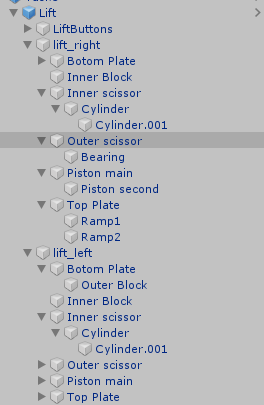
\includegraphics[width=1\textwidth]{fig/phase_2/implementation/carliftTreee.PNG}
    \caption{Hierarchy of \textit{Lift} prefab.}
    \label{fig:carliftTree}
  \end{subfigure}
  \hfill%
  \caption{The car lift prefab from the garage scene.}
  \label{fig:phase2CarLift}
\end{figure}


\subsection{Optimisation} \label{subsec:Optimisation}
Over the course of the implementation of the artefacts, areas that could be improved and bugs that could be fixed appeared. As they were noticed, or certain parts caused issues, the issues were taken note of and general implementation continued. If a bug or piece of code was hindering the implementation it would be fixed as needed, otherwise left for later. At the tail end of the phase, they were prioritised and ordered, and they could then be fixed, one at a time. Among these were improvements to level loading, missing collision detectors for certain items, incorrectly synchronised objects, etc. Multiple passes were made to make sure that remote procedure calls were not being sent multiple times or being looped by firing other users' event handlers and so on. 

A helper method has also been created to help keep the code general. Instead of creating a new remote procedure call every time one is needed, one can simply pass the desired method call as a argument to the helper, and the method will initiate the desired remote procedure call. We also optimised which remote clients gets the RPC call, reducing network traffic and complexity. For instance we could specifically target the \textit{MasterClient}, the \textit{others} (all but the masterclient) or simply every remote client connected.     



\subsection{Challenges}
One of the more complex challenges encountered was the fact that the workplace being revamped to function with multiple users was simply not designed from the start with this in mind. This meant that certain scripts needed to be altered to function while networked, and a discussion was had regarding the validity of the tasks as collaborative work. However, as mentioned in section \ref{section:CSCL}, the act of collaborating in itself can bring about better learning through simply discussing and bouncing ideas off another person. A task need not necessarily be created for multiple users for a group to gain benefits from solving it together.

\subsubsection{Covid-19 pandemic}
\label{section:covid19}
Due to the global corona virus pandemic (Covid-19) and restrictions issued by the Norwegian government as part of their actions to prevent spread of the disease \cite{FhiCorona} impediments arose. Social distancing, isolation and the considerable risk of transferring the virus from the VR headsets and controllers meant that the VR lab at the university was closed until further notice and that scheduled testing with the primary target group could not be carried out as planned. Although some user testing was completed before the restrictions, we did not manage to get enough satisfactory results. More about this in section \ref{section:secondEvalPhase2}. It became clear that proper data collection to answer Secondary RQ1 (see section \ref{RQ}) was not feasible, as it meant we would need both counsellor and job seekers using VR equipment they do not have at home or be localised at the VR lab at the same time which was not permitted. However, we did plan to run test for data collection with both peers and mentors. Further details of plan is described in section \ref{section:secondEvalPhase2}.

As discussed with our supervisors in the preliminary phase of the pandemic we decided to add a research question which shifts focus to remote collaboration as a career guidance tool. However, we consider the RQ1 as potential future work, see section \ref{section:futureWork} for more. 

Covid-19 also meant we had continue work from home by setting up temporary VR stations in our apartments. Relatively small areas were not ideal for tracking and movement, but we adapted to the situation. As for the VR equipment, it was borrowed from the IMTEL lab, specifically an Oculus Rift and Rift S. We therefore had to accommodate to new controller bindings and setup as we previously mainly worked on HTC Vive and Index, i.e. non-Oculus devices.            





\section{Second Evaluation}
\label{section:secondEvalPhase2}
In order to evaluate the usability of the application and collaborative features we developed for this phase we utilised a reliable and well established method called system usability scale (SUS). The scale gives a number representing a composite measure of the overall usability of the system being studied \cite{brooke1996sus}. In order for SUS to have the best result it is important that the test is performed before any discussion around the trial of the system takes place, which we tried our best to ensure.

The SUS questions were translated in the testers' native language (Norwegian) and included in a separate category in a survey, amongst two other likert scale categories related to career guidance/career choice and collaboration mechanisms. This is a popular strategy for user evaluation of a computer system \cite{oates2005researching}. Some of the questions were adapted and utilised from an evaluation system designed by an associate professor from the Department of Education and Lifelong Learning at NTNU. Questions about career guidance, engagement and self-efficacy measurements aimed to answer the primary RQ. SUS provides answers for usability, e.g. secondary RQ2. Comparing feedback from seeker-seeker vs. seeker-counsellor would provide answers to secondary RQ1.  The survey can be found in appendix \ref{appendix:phase2}.

The plan for the user testing was to conduct twelve separate tests with pairs of two. Either seeker-seeker or seeker-mentor would try out the application in VR before answering the survey. This meant we would have 24 answers, half of which was seeker-seeker pairs and the other half seeker and mentor. The  mentors would be career counsellors from NAV Jobbhuset Falkenborg. Figure \ref{fig:tastingPhase2} shows a job seeker equipped with HTC Vive testing the application and the experience once inside the virtual environment. 


\begin{figure}[]
  \centering
   \captionsetup{width=.9\linewidth}
    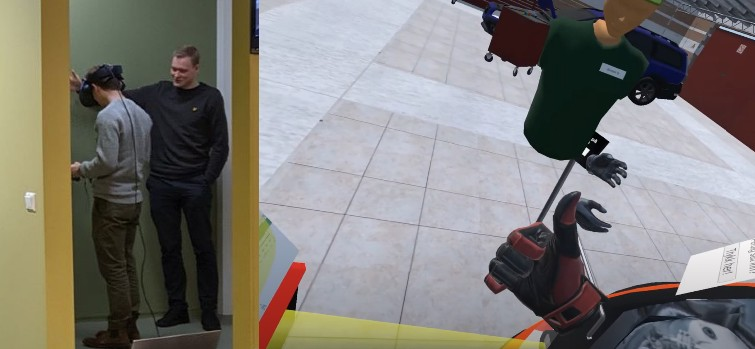
\includegraphics[width=0.9\textwidth]{fig/phase_2/phase2_testing.jpg}
 \caption{User testing in progress at the IMTEL lab and the users perspective inside the application.}
\label{fig:tastingPhase2}
\end{figure}


\subsection{User test data}
As mentioned in the challenges we faced for this phase, the Covid-19 pandemic meant that we were not able to complete our planned testing. We were only able to conduct six tests, i.e. \textit{3*2} pairs of job seekers, thus missing the other half of counsellors and seekers. Ideally we would have gotten the last half and from there we could  compare the data sets of the two halves. Therefore it meant we could not evaluate what the effects of collaborating in virtual reality with another job seeker compared to a counsellor were. At the time of writing, the restrictions are still in effect leaving us unable to properly discuss and answer the Secondary RQ1. The testing started in March 2020, see table \ref{table:dataGatheringSchedule}.     


\subsection{Analysis}
Although we did not complete the user testing, we still got half of the intended data points, and they will be presented here. An important note is that we cannot definitely conclude or properly discuss using these results as they are incomplete and the number of answers is not enough for quantitative analysis.  We will present key and interesting findings, as they still hold some good value for the thesis. 

%Since we used a survey as the data gathering method the results are based on measure quantities of those primary users participating and not subjective opinions which means that potential findings still hold some good value for the thesis.       

\subsubsection{Quantitative Data Analysis}
In order to get meaningful information from the quantitative data we utilised different techniques to help manage, view and analyse it. The survey mainly consisted of likert scales, which is an ordinal data type, meaning the numbers are allocated to a quantitative scale \cite{oates2005researching}. The full survey and answers can found in appendix \ref{appendix:phase2}. In our survey they were asked to answer to what degree they agreed with statements regarding VR on a scale from 1-5, where 1 is "Low degree" and 5 was "High degree". The survey had nominal data points as well which describes categories instead of number or scale, such as Yes/No questions. Finally, interval data type was used in regards to the age of the users, where measurement is along a scale but the points on the scale intervals with a fixed number such as the age intervals: 10-20, 21-30, 31-40. 

Through organisation of the data by using visual aids and statistics we were able to identify interesting findings. The survey had six answers consisting of one woman and five males with age distribution 18-25 years. Of those, none had tried NAV VR applications before. Data results are presented in bar charts and was constructed using an online graph maker. 


\begin{figure}[]
  \begin{subfigure}[b]{0.5\textwidth}
    \captionsetup{width=0.8\linewidth}
    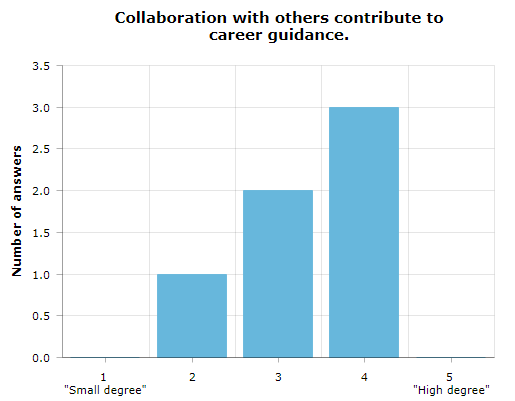
\includegraphics[width=1\textwidth]{fig/phase_2/charts/collabIncreaseCareer.PNG}
    \caption{}
    \label{fig:phase2_collabIncreaseCareer}
  \end{subfigure}
  \hfill%
  \begin{subfigure}[b]{0.5\textwidth}
    \captionsetup{width=0.8\linewidth}
    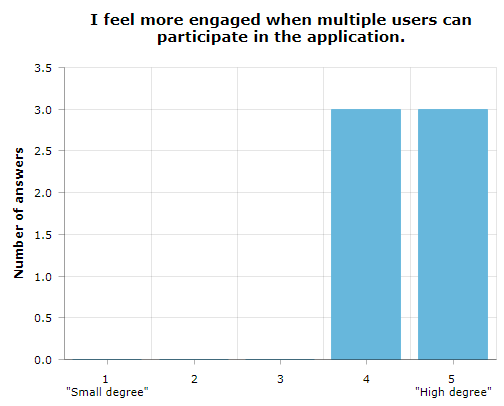
\includegraphics[width=1\textwidth]{fig/phase_2/charts/collabMoreEngaged.PNG}
    \caption{}
    \label{fig:phase2_collabMoreEngaged}
  \end{subfigure}
  \hfill%
  \begin{subfigure}[b]{0.5\textwidth}
    \captionsetup{width=0.8\linewidth}
    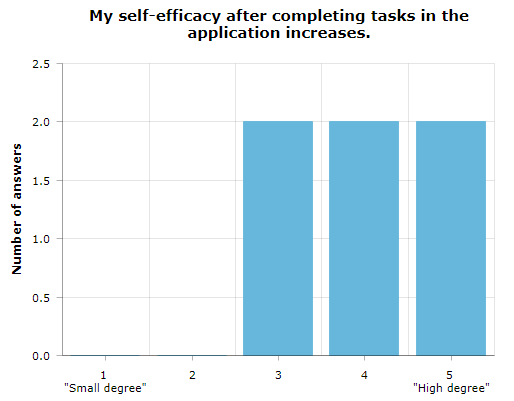
\includegraphics[width=1\textwidth]{fig/phase_2/charts/collabSelfEfficacy.PNG}
    \caption{}
    \label{fig:phase2_collabSelfEfficacy}
  \end{subfigure}
  \hfill%
  \begin{subfigure}[b]{0.5\textwidth}
    \captionsetup{width=0.8\linewidth}
    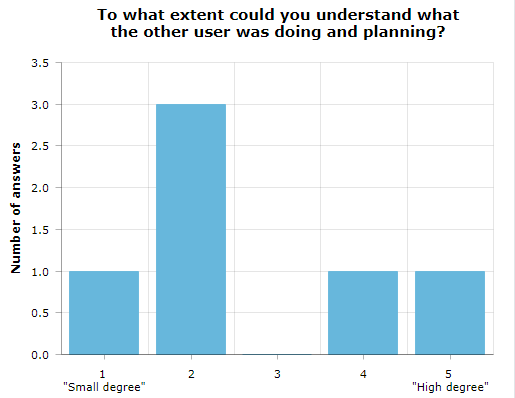
\includegraphics[width=1\textwidth]{fig/phase_2/charts/collabPlanningDoing.PNG}
    \caption{}
    \label{fig:phase2_collabPlanning}
  \end{subfigure}
  \caption{Bar charts showing the participants likert scale answers to various statements.}
  \label{fig:phase2_allCharts}
\end{figure}

There was a general consensus that the addition of collaboration mechanisms in the virtual reality application contributed with a positive effect in terms of increasing the engagement of the users and their career guidance, see figure \ref{fig:phase2_collabIncreaseCareer} and \ref{fig:phase2_collabMoreEngaged}. Figure \ref{fig:phase2_collabMoreEngaged} shows that 50\% rated 5, "High degree" (\textit{High degree}) and the other 50\% rated 4. Figure \ref{fig:phase2_collabIncreaseCareer}  shows the mode is 4 on the scale. 
An important aspect according to employees at NAV is that several young job seekers lack a sense of achievement. The responses from the testing show that they obtain just this after completing tasks in the application, such as adjusting the headlights of a car, increasing the individual's belief in her or him, i.e. their sense of self-efficacy. Figure \ref{fig:phase2_collabSelfEfficacy} shows that 66.66\% (or 2/3) agree or highly agree that their self-efficacy increases. The mean and median being 4 on the scale, which is \textit{Agree}. 

There was however divided opinions in regards to whether or not they understood what the other user was doing or planning to do. Figure \ref{fig:phase2_collabPlanning} shows that only one third (33.33\%) rated 4 or 5, whereas two thirds (66.66\%) ranked 1 or 2. The mode being 2. It is therefore clear that the users feeling of social presence in VR can vary from person to person. 

We must also consider the limitations of this survey which does not have enough data entries and lacks testing with a career counsellor. It does however have the correct target group which is part of why we included it, since due to the Covid-19 situation it proved difficult to to run such a test again with the desired test audience.


\subsubsection{SUS Score}
\label{section:phase2SUS}
In order interpret the system usability scale (SUS) score we needed to calculate the score for each participant, which gives a number from 0-100. This will result in a score which can be used as an interpretation of the usability performance of the system in the aspects of effectiveness, efficiency, and overall ease of use \cite{SusMeasuringInterpret}. However, we wanted to get the average SUS score, which we simply got by adding all individual scores and divided by the number of scores. The following steps is required for each score calculation: 


\begin{enumerate}
  \item Converted each scale into points for all ten answers, see Table \ref{table:SUSconversionPoints}. 
  \item Calculate X. \textit{X = sum of the points for all odd-numbered questions – 5}  
  \item Calculate Y. \textit{Y =  25 – Sum of the points for all even-numbered questions}
  \item Calculate SUS score. \textit{SUS Score =} $(X + Y) * 2.5$ 
\end{enumerate}


\begin{table}[H]
\centering
\begin{tabular}{l|l}
{ \textbf{Scale}} & { \textbf{Point}} \\ \hline
Strongly Disagree                     & 1                                     \\ 
Disagree                              & 2                                     \\ 
Neutral                               & 3                                     \\ 
Agree                                 & 4                                     \\ 
Strongly Agree                        & 5                                     \\ 
\end{tabular}
\caption{SUS scale/point conversion table.}
\label{table:SUSconversionPoints}
\end{table}

Using this method we calculated the SUS score for each of the participants. The results can be found in table \ref{table:SUSscores}. This gives an average SUS score of: 

\[\overline{SUS} = \frac{68 + 32.5 + 42.5 + 82.25 + 85 + 70}{6} = \frac{379.25}{6} \approx 63.2\]

According to table \ref{table:SUSinterpret} this results in a \textit{Poor} adjective rating of the usability for the collective participants. The average SUS score is 68 \cite{SusMeasuringInterpret}. However, due the number of data entries being low (six participants) the average score is highly affected by scores which are very low or opposite. The median SUS score 69, which correlates to a \textit{Good} rating and is above the average SUS score. Also interesting is the number of the SUS scores and their coherent adjective rating. Here we find 2 scores in the \textit{Excellent} rating, 1 in the \textit{Good} rating, 2 in the \textit{Okay} rating, and finally 2 in \textit{Awful} rating. This shows that there is divided opinions about the usability of such an VR application. This may have some correlation with the fact that non of the users had tried had tried NAV VR applications before and that they had limited experience with VR. 




\begin{table}[H]
\centering
\begin{tabular}{l|l}
{ \textbf{Participant ID}} & { \textbf{SUS score}} \\ \hline
2   & 32.5                                     \\ 
3   & 42.5                                    \\ 
1   & 68                                   \\ 
6   & 70                                     \\ 
4   & 82.25                                    \\ 
5   & 85                                     \\ 
\end{tabular}
\caption{SUS scores for each participant sorted ascending by score.}
\label{table:SUSscores}
\end{table}


\begin{table}[H]
\centering
\begin{tabular}{l|l|l}
{ \textbf{SUS score}} & { \textbf{Grade}} & { \textbf{Adjective rating}} \\ \hline
$>$ 80.3   & A &  Excellent                                 \\ 
68 – 80.3   & B & Good                                  \\ 
68   & C   &   Okay                              \\ 
51 – 68   & D   &  Poor                               \\ 
$<$ 51  & F      &     Awful                         \\ 
\end{tabular}
\caption{SUS scores and their rating \cite{SusMeasuringInterpret}.}
\label{table:SUSinterpret}
\end{table}



\subsubsection{Visibility}
\label{section:phase2visibility}
As presented in the analysis the feeling of presence, e.g. the feeling of being in the VR environment, varied quite a lot, see figure \ref{fig:phase2_collabPlanning}. There are a number of factors including technological, user and interaction variables that influences presence \cite{oh2018systematic} \cite{presenceInVirtualReality:}. Technical variables such as display resolution or consistent sensor inputs may have an impact on the users and should considered. Also, the degree of interaction in the application can influence the presence as it can focus their attention and result in increased involvement \cite{presenceInVirtualReality:}. 
Some participants pointed out after the testing that the voice communication worked well, but they had some difficulty identifying who talked and when. This may be optimised by speech indicators, such as an speaker symbol over the avatar, or other animations.     

\subsubsection{Remote career guidance}
%lobby + 16players + desktop version
Due to the new situation regarding the virus pandemic we added a new research question which shifts focus to remote career guidance. As such, a complete lobby system, with hosting, creation and selection of different application should be created for the next phase. While it may restrict our time and ability to develop other features it provides a unique opportunity for testing and demonstration over the network across the country or even worldwide.   


%**Primary RQ: [Valgkompetanse]**
%(1) self-efficacy measurements
%(2) career guidence (valgkompetanse)
%(3) engagement

%**Secondary RQ1:**
%(1) compare feedback from [Peers+Peer] vs. [Peers+Mentor]

%**Secondary RQ2: [Samarbeidsmekanismer]**
%(1) Usability testing (System Usability Scale SUS)



%Primary RQ:
%“How does collaboration in virtual reality (VR) workplaces contribute to the careerguidance of young job seekers?”

%Secondary RQ1:
%“What are the effects of collaborating in virtual reality (VR) with a mentor comparedto a peer?”

%Secondary RQ2:
%”What is essential for collaborative virtual reality to be applied effectively for remotecareer guidance?”

%Secondary RQ3:
%”What type of collaborative features are technically feasible for workplace experi-ence in a virtual environment?”

%Secondary RQ4:
%”What  are  the  challenges  of  implementing  collaborative  features  in  an  ongoingproject?


\subsubsection{Considerations for the next survey}
Due to the fact that our primary testing target group became mostly unavailable for a unknown amount of time we must be wary of the effect on the data generation in the next phase.  Considerations should include how the users experienced the application and how the testing is conducted.

\cleardoublepage